%% Admitere Fizică FA Varianta A, 2015-2019 %%

\section{Admitere Fa iulie 2019}

2019.A.1. Un sistem termodinamic închis efectuează un lucru mecanic de $200 \mathrm{~J}$ şi primeşte o cantitate de căldură de $600 \mathrm{~J}$. Variația energiei interne a sistemului este: (6pct.)\\ a) $600 \mathrm{~J}$; b) $400 \mathrm{~J}$; c) $300 \mathrm{~J}$; d) $-800 \mathrm{~J}$; e) $800 \mathrm{~J}$; f) $-600 \mathrm{~J}$.\\ dr. Savu-Sorin Ciobanu\\ Variația energiei interne este diferenţa dintre căldura primită şi lucrul mecanic efectuat: $\Delta \mathrm{U}=\mathrm{Q}-\mathrm{L}=400 \mathrm{~J}$. Răspuns corect b).\\

2019.A.2. Un mol de gaz ideal cu căldura molară la volum constant $\mathrm{C}_{\mathrm{v}}=3 \mathrm{R} / 2$ suferă o transformare descrisă de relaţia $\mathrm{T}=\mathrm{aV}^{2}$, unde $a$ este o constantă pozitivă. Căldura molară în această transformare este: (6pct.)\\ a) $5 R / 2$; b) $R$; c) $3 R / 2$; d) $R / 2$; e) $2 R$; f) $3 R$.\\ dr. Savu-Sorin Ciobanu\\ Folosind ecuaţia termică de stare a gazului ideal $\mathrm{pV}=\nu \mathrm{RT}$ şi ecuaţia transformării suferite de gazul ideal $T=a V^{2}$, obţinem $p V=\nu R a V^{2}$, adică $p=b V$, unde $b=\nu R a$ este tot o constantă pozitivă.\\ În coordonate $\mathrm{p}-\mathrm{V}$, transformarea gazului este descrisă de o dreaptă care trece prin origine. Considerând transformarea între stările iniţială şi finală de temperaturi $\mathrm{T}_{\mathrm{i}}$ şi $\mathrm{T}_{\mathrm{f}}$, după calcularea variaţiei energiei interne $\Delta U=\nu C_{v}\left(T_{f}-T_{i}\right)$ şi a lucrului mecanic efectuat de gaz $L=\frac{p_{f}+p_{i}}{2}\left(V_{f}-V_{i}\right)=\frac{b}{2}\left(V_{f}^{2}-V_{i}^{2}\right)=\nu \frac{R}{2}\left(T_{f}-T_{i}\right)$, folosind $Q=\Delta U+L$ şi definiţia căldurii molare $\mathrm{C}=\frac{\mathrm{Q}}{\nu\left(\mathrm{~T}_{\mathrm{f}}-\mathrm{T}_{\mathrm{i}}\right)}$, se obţine căldura molară a gazului în această transformare: $\mathrm{C}=\mathrm{C}_{\mathrm{v}}+\frac{\mathrm{R}}{2}=2 \mathrm{R}$. Răspuns corect e).\\

2019.A.3. Printr-un rezistor cu rezistenţa $\mathrm{R}=40 \Omega$ trece un curent cu intensitatea $\mathrm{I}=5 \mathrm{~A}$. Energia disipată pe rezistor în timp de o oră este: (6pct.)\\ a) $7,2 \mathrm{~MJ}$; b) $100 \mathrm{~kJ}$; c) $3,6 \mathrm{~kJ}$; d) $3,6 \mathrm{~MJ}$; e) $7,2 \mathrm{~kJ}$; f) $20 \mathrm{~kJ}$.\\ dr. Savu-Sorin Ciobanu\\ Energia degajată de rezistor este $W=\mathrm{RI}^{2} t=3,6 \mathrm{~MJ}$. Răspuns corect d).\\

2019.A.4. Într-un circuit simplu format dintr-o sursă cu tensiunea electromotoare $\mathrm{E}=12 \mathrm{~V}$, rezistenţa internă $\mathrm{r}=0,5 \Omega$ şi un rezistor cu rezistenţa $\mathrm{R}=5,5 \Omega$, intensitatea curentului este: (6pct.)\\ a) $6 \mathrm{~A}$; b) $24 \mathrm{~A}$; c) $4 \mathrm{~A}$; d) $2 \mathrm{~A}$; e) $0,5 \mathrm{~A}$; f) $3 \mathrm{~A}$.\\ dr. Savu-Sorin Ciobanu\\ Avem $\mathrm{I}=\frac{\mathrm{E}}{\mathrm{R}+\mathrm{r}}=2 \mathrm{~A}$. Răspuns corect d).\\

2019.A.5. Un corp cu masa de $0,5 \mathrm{~kg}$ se află în repaus la înălțimea de $0,5 \mathrm{~m}$ faţă de sol. Energia potențială a corpului în câmp gravitaţional ($\mathrm{g}=10 \mathrm{~m} / \mathrm{s}^{2}$) este: (6pct.)\\ a) $5 \mathrm{~J}$; b) $0,5 \mathrm{~J}$; c) $0,25 \mathrm{~J}$; d) $25 \mathrm{~mJ}$; e) $2,5 \mathrm{~J}$; f) $25 \mathrm{~J}$.\\ dr. Savu-Sorin Ciobanu\\ Energia potențială este $\mathrm{E}_{\mathrm{p}}=\mathrm{mgh}=2,5 \mathrm{~J}$. Răspuns corect e).\\

2019.A.6. Randamentul unei maşini termice care funcţionează după un ciclu Carnot între temperaturile $300 \mathrm{~K}$ şi $800 \mathrm{~K}$ este: (6pct.)\\ a) $62,5 \%$; b) $80 \%$; c) $87,5 \%$; d) $37,5 \%$; e) $42,5 \%$; f) $30 \%$.\\ dr. Savu-Sorin Ciobanu\\ Randamentul este: $\eta=1-\frac{\mathrm{T}_{\mathrm{r}}}{\mathrm{T}_{\mathrm{c}}}=1-\frac{300 \mathrm{~K}}{800 \mathrm{~K}}=\frac{5}{8}=62,5 \%$. Răspuns corect a).\\

2019.A.7. Un rezistor cu rezistenţă variabilă este alimentat de 4 baterii identice legate în serie, fiecare cu tensiunea electromotoare $\mathrm{E}=1,5 \mathrm{~V}$ şi rezistenţa internă $\mathrm{r}=0,3 \Omega$. Valoarea maximă a puterii ce poate fi debitată pe rezistor este: (6pct.)\\ a) $30 \mathrm{~W}$; b) $15 \mathrm{~W}$; c) $12 \mathrm{~W}$; d) $7,5 \mathrm{~W}$; e) $1,2 \mathrm{~W}$; f) $6 \mathrm{~W}$.\\ dr. Savu-Sorin Ciobanu\\ Gruparea bateriilor are tensiunea electromotoare echivalentă $E_{e}=4 E=6 V$ şi rezistenţa internă echivalentă $r_{e}=4 r=1,2 \Omega$.\\ Pentru o valoare a rezistenței exterioare egală cu $r_{e}$ se degajă o putere maximă pe rezistor $P_{\max}=r_{e} \frac{E_{e}^{2}}{\left(2 r_{e}\right)^{2}}=7,5 \mathrm{~W}$. Răspuns corect d ).\\

2019.A.8. Rezistenţa echivalentă a doi rezistori cu rezistenţele $\mathrm{R}_{1}=4 \Omega$ și $\mathrm{R}_{2}=12 \Omega$ legaţi în paralel este: (6pct.)\\ a) $4 \Omega$; b) $8 \Omega$; c) $6 \Omega$; d) $16 \Omega$; e) $10 \Omega$; f) $3 \Omega$.\\ dr. Savu-Sorin Ciobanu\\ Folosind $\frac{1}{\mathrm{R}_{\mathrm{e}}}=\frac{1}{\mathrm{R}_{1}}+\frac{1}{\mathrm{R}_{2}}$, se obţine $\mathrm{R}_{\mathrm{e}}=3 \Omega$. Răspuns corect f).\\

2019.A.9. Trei corpuri de mase $m_{1}=m_{2}=3 m_{3}$ sunt legate printr-un fir ideal trecut peste trei scripeţi ideali ca în figură. Valoarea absolută a raportului acceleraţiilor corpurilor de masă $m_{1}$ şi $m_{3}$ este: (6pct.)\\ a) $1$; b) $2 / 3$; c) $4$; d) $1 / 3$; e) $2$; f) $4 / 3$.\\ dr. Savu-Sorin Ciobanu\\ 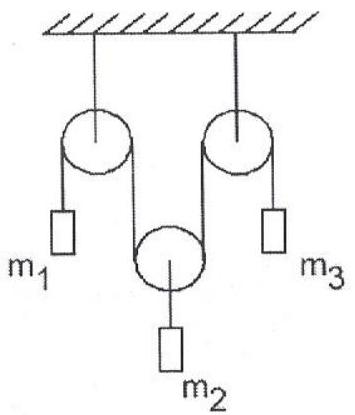
\includegraphics[width=0.4\linewidth]{images/2025_08_19_7d65f00c22d2f38e2422g-02}\\ Comparând masele corpurilor, tragem concluzia că $m_{3}$ urcă, $m_{2}$ urcă şi $m_{1}$ coboară, cu valorile absolute ale acceleraţiilor $a_{3}$, $a_{2}$ şi $a_{1}$. Cum firul este ideal, tensiunea este aceeaşi în tot firul. Astfel, legea a doua a dinamicii pentru cele trei corpuri se scrie:\\ $\mathrm{T}-\mathrm{m}_{3} \mathrm{~g}=\mathrm{m}_{3} \mathrm{a}_{3}$;\\ $\mathrm{m}_{1} \mathrm{~g}-\mathrm{T}=\mathrm{m}_{1} \mathrm{a}_{1}$;\\ $2 \mathrm{~T}-\mathrm{m}_{2} \mathrm{~g}=\mathrm{m}_{2} \mathrm{a}_{2}$.\\ Cum la o urcare cu distanța $x$ a corpului 3, fără ca corpul 1 să se mişte, corpul 2 coboară cu $x / 2$ (evident, în acelaşi timp), iar la o coborâre cu distanţa $x$ a corpului 1, fără ca corpul 3 să se miște, corpul 2 urcă cu $x / 2$ (sau mai general, la o urcare cu distanţa $\mathrm{x}_{3}$ a corpului 3 şi la o coborâre cu distanţa $x_{1}$ a corpului 1 într-un interval de timp dat, corpul 2 urcă cu o distanţă $x_{2}=\frac{x_{1}-x_{3}}{2}$), obţinem:\\ $\mathrm{a}_{2}=\frac{\mathrm{a}_{1}-\mathrm{a}_{3}}{2}$.\\ Exprimând $T$ dintr-una din primele 3 ecuaţii şi înlocuind în celelalte două, şi folosind şi cea de-a patra ecuaţie, obţinem un sistem de 3 ecuaţii liniare cu 3 necunoscute, $a_{1}$, $a_{2}$ și $a_{3}$, care are soluţiile:\\ $\mathrm{a}_{1}=\mathrm{g} / 2$, $\mathrm{a}_{2}=0$, $\mathrm{a}_{3}=\mathrm{g} / 2$.\\ În final, $\frac{\mathrm{a}_{1}}{\mathrm{a}_{3}}=1$. Comparând cu consideraţiile iniţiale, constatăm că $m_{3}$ într-adevăr urcă, $m_{1}$ într-adevăr coboară, iar $\mathrm{m}_{2}$ are o acceleraţie nulă, deci dacă viteza sa iniţială este nulă, rămâne în repaus. Răspuns corect a).\\

2019.A.10. Racheta Saturn folosită în programul Apollo genera o forţă de propulsie de $35 \mathrm{~MN}$. Ştiind că masa rachetei era de $2800$ de tone, acceleraţia acesteia după lansare a fost ($\mathrm{g}=10 \mathrm{~m} / \mathrm{s}^{2}$): (6pct.)\\ a) $10 \mathrm{~m} / \mathrm{s}^{2}$; b) $28 \mathrm{~m} / \mathrm{s}^{2}$; c) $7 \mathrm{~m} / \mathrm{s}^{2}$; d) $35 \mathrm{~m} / \mathrm{s}^{2}$; e) $2,5 \mathrm{~m} / \mathrm{s}^{2}$; f) $3,5 \mathrm{~m} / \mathrm{s}^{2}$.\\ dr. Savu-Sorin Ciobanu\\ Lansarea fiind pe verticală, acceleraţia rachetei este:\\ $\mathrm{a}=\frac{\mathrm{F}-\mathrm{mg}}{\mathrm{m}}=\frac{\mathrm{F}}{\mathrm{m}}-\mathrm{g}=2,5 \mathrm{~m} / \mathrm{s}^{2}$. Răspuns corect e).\\

2019.A.11. Un corp cu masa de $2 \mathrm{~kg}$ are viteza $10 \mathrm{~m} / \mathrm{s}$. Impulsul corpului este: (6pct.)\\ a) $100 \mathrm{~N} \cdot \mathrm{~s}$; b) $5 \mathrm{~N} \cdot \mathrm{~s}$; c) $50 \mathrm{~N} \cdot \mathrm{~s}$; d) $10 \mathrm{~N} \cdot \mathrm{~s}$; e) $20 \mathrm{~N} \cdot \mathrm{~s}$; f) $2 \mathrm{~N} \cdot \mathrm{~s}$.\\ dr. Savu-Sorin Ciobanu\\ Impulsul este: $\mathrm{p}=\mathrm{mv}=20 \mathrm{~kg} \cdot \mathrm{m} / \mathrm{s}=20 \mathrm{~N} \cdot \mathrm{s}$. Răspuns corect e).\\

2019.A.12. Un mobil cu masa $\mathrm{m}=200 \mathrm{~g}$ se mişcă după legea $\mathrm{x}(\mathrm{t})=4+2 \mathrm{t}+2 \mathrm{t}^{2}$ (x este măsurat în metri, iar $t$ în secunde). Energia cinetică a mobilului la momentul $t=2 \mathrm{~s}$ este: (6pct.)\\ a) $4 \mathrm{~J}$; b) $1 \mathrm{~J}$; c) $10 \mathrm{~J}$; d) $30 \mathrm{~J}$; e) $2 \mathrm{~J}$; f) $20 \mathrm{~J}$.\\ dr. Savu-Sorin Ciobanu\\ Viteza mobilului este $\mathrm{v}(\mathrm{t})=\frac{\mathrm{dx}}{\mathrm{dt}}=2+4 \mathrm{t}$, deci $\mathrm{v}(2)=10 \mathrm{~m} / \mathrm{s}$ şi $\mathrm{E}_{\mathrm{c}}=\frac{\mathrm{mv}^{2}}{2}=10 \mathrm{~J}$. Răspuns corect c).\\

2019.A.13. În SI unitatea de măsură pentru căldura specifică este: (6pct.)\\ a) $\mathrm{J} \cdot \mathrm{K}^{-1}$; b) $\mathrm{J} \cdot \mathrm{kg}^{-1} \cdot \mathrm{~K}$; c) $\mathrm{J} \cdot \mathrm{kg}^{-1}$; d) $\mathrm{J} \cdot \mathrm{mol}^{-1} \cdot \mathrm{~K}^{-1}$; e) $\mathrm{J} \cdot \mathrm{kg}^{-1} \cdot \mathrm{~K}^{-1}$; f) $\mathrm{J} \cdot \mathrm{kg} \cdot \mathrm{K}^{-1}$.\\ dr. Savu-Sorin Ciobanu\\ Din definiţie $\mathrm{c}=\frac{\mathrm{Q}}{\mathrm{m} \Delta \mathrm{T}}$, deci $\left[\mathrm{c}\right]_{\mathrm{SI}}=\frac{\mathrm{J}}{\mathrm{kg} \cdot \mathrm{K}}$. Răspuns corect e).\\

2019.A.14. În circuitul din figură se cunosc $\mathrm{R}_{1}=3 \Omega$ şi $\mathrm{R}_{2}=9 \Omega$. Rezistenţa echivalentă între punctele A şi B este: (6pct.)\\ a) $7,5 \Omega$; b) $4,5 \Omega$; c) $6 \Omega$; d) $5 \Omega$; e) $2,5 \Omega$; f) $6,5 \Omega$.\\ dr. Savu-Sorin Ciobanu\\ 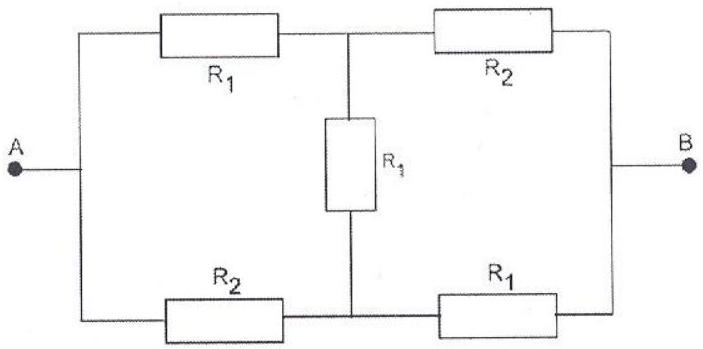
\includegraphics[width=0.4\linewidth]{images/2025_08_19_7d65f00c22d2f38e2422g-04(1)}\\ Considerăm că se pune o tensiune electrică $\mathrm{U}_{\mathrm{AB}}$ între punctele A și B, cu borna pozitivă pe A şi cea negativă pe B. În acest caz curenţii electrici care trec prin gruparea de rezistenţe se figurează astfel:\\ \begin{center} 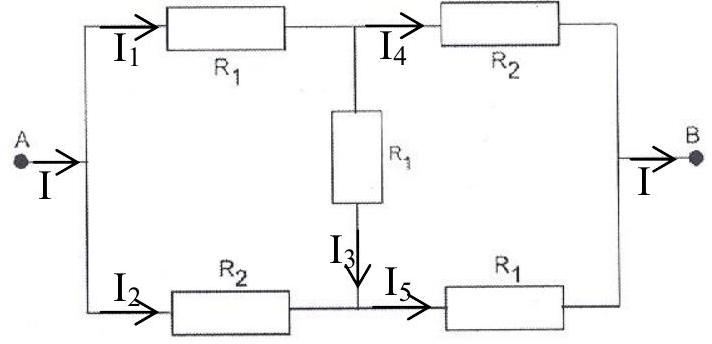
\includegraphics[width=0.4\linewidth]{images/2025_08_19_7d65f00c22d2f38e2422g-04(2)} \end{center}\\ Folosim acum simetria montajului de rezistoare. Astfel, rotind figura cu $180^{\circ}$:\\ \begin{center} 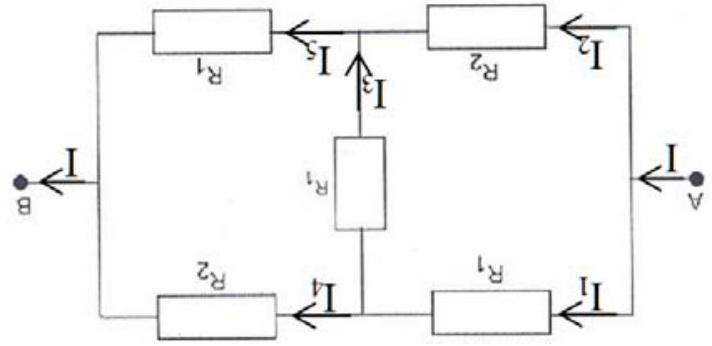
\includegraphics[width=0.4\linewidth]{images/2025_08_19_7d65f00c22d2f38e2422g-04} \end{center}\\ Eventual desenând-o pe o altă hârtie, observăm mai întâi curenţii, apoi punem tensiunea electrică $\mathrm{U}_{\mathrm{AB}}$ cu borna pozitivă pe B (care acum a ajuns în stânga), deci schimbăm sensul tuturor curenţilor. Constatăm că avem aceeaşi figură ca la început (borna B este vechea bornă A şi invers), şi că: $\mathrm{I}_{5}=\mathrm{I}_{1}$, $\mathrm{I}_{4}=\mathrm{I}_{2}$.\\ Folosind aceste rezultate, refacem prima figură:\\ \begin{center} 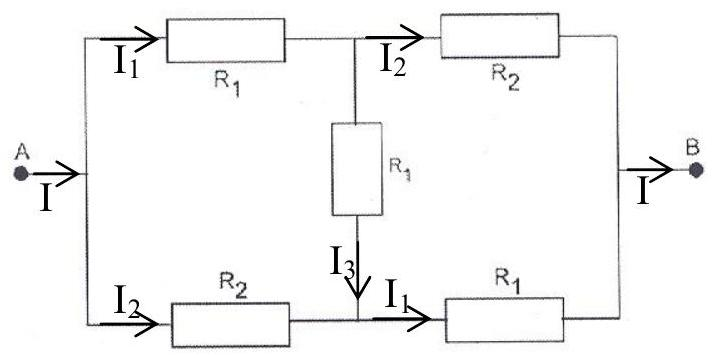
\includegraphics[width=0.4\linewidth]{images/2025_08_19_7d65f00c22d2f38e2422g-05} \end{center}\\ Folosind legile lui Kirchhoff, avem:\\ $\mathrm{I}=\mathrm{I}_{1}+\mathrm{I}_{2}$;\\ $\mathrm{I}_{1}=\mathrm{I}_{2}+\mathrm{I}_{3}$;\\ $\mathrm{I}_{1} \mathrm{R}_{1}+\mathrm{I}_{3} \mathrm{R}_{1}=\mathrm{I}_{2} \mathrm{R}_{2}$.\\ Din ultimele două ecuaţii obţinem:\\ $\mathrm{I}_{2}=\frac{2 \mathrm{I}_{1} \mathrm{R}_{1}}{\mathrm{R}_{1}+\mathrm{R}_{2}}$;\\ $I_{3}=\frac{I_{1}\left(R_{2}-R_{1}\right)}{R_{1}+R_{2}}$.\\ Avem, folosind semnificaţia rezistenţei echivalente între punctele A şi B:\\ $\mathrm{U}_{\mathrm{AB}}=\mathrm{R}_{\mathrm{e}} \mathrm{I}=\mathrm{R}_{\mathrm{e}}\left(\mathrm{I}_{1}+\mathrm{I}_{2}\right)=\mathrm{R}_{\mathrm{e}} \mathrm{I}_{1} \frac{3 \mathrm{R}_{1}+\mathrm{R}_{2}}{\mathrm{R}_{1}+\mathrm{R}_{2}}$\\ Și de asemenea, folosind drumul dintre punctele A şi B format din laturile din partea de sus a grupării:\\ $\mathrm{U}_{\mathrm{AB}}=\mathrm{R}_{1} \mathrm{I}_{1}+\mathrm{R}_{2} \mathrm{I}_{2}=\mathrm{R}_{1} \mathrm{I}_{1} \frac{\mathrm{R}_{1}+3 \mathrm{R}_{2}}{\mathrm{R}_{1}+\mathrm{R}_{2}}$.\\ Deci rezistenţa echivalentă între punctele $A$ şi $B$ este:\\ $R_{e}=R_{1} \frac{R_{1}+3 R_{2}}{3 R_{1}+R_{2}}=5 \Omega$. Răspuns corect d).\\

2019.A.15. Un gaz ideal se destinde adiabatic. În cursul procesului volumul creşte de $100$ ori iar temperatura scade de $10$ ori. Exponentul adiabatic al gazului este: (6pct.)\\ a) $4 / 3$; b) $2$; c) $7 / 5$; d) $3 / 2$; e) $6 / 5$; f) $5 / 4$.\\ dr. Savu-Sorin Ciobanu\\ Legea transformării adiabatice este $\mathrm{TV}^{\gamma-1}=\mathrm{ct}=\mathrm{T}_{\mathrm{i}} \mathrm{V}_{\mathrm{i}}^{\gamma-1}=\mathrm{T}_{\mathrm{f}} \mathrm{V}_{\mathrm{f}}^{\gamma-1}$. Folosind şi datele din enunţ scriem $\left(\frac{V_{f}}{V_{i}}\right)^{\gamma-1}=100^{\gamma-1}=\frac{T_{i}}{T_{f}}=10$. Deci exponentul adiabatic al gazului este $\gamma=1,5$. Răspuns corect d).

\section{Admitere Fa iulie 2018}

2018.A.1. Un corp este lansat cu viteza initială de $10 \mathrm{~m} / \mathrm{s}$ pe un plan orizontal. Coeficientul de frecare la alunecare dintre corp şi plan este $0,2$. Timpul după care corpul se opreşte este $\left(g=10 \mathrm{~m} / \mathrm{s}^{2}\right)$ : (6 pct.)\\ a) $5 \mathrm{~s}$; b) $2 \mathrm{~s}$; c) $1 \mathrm{~s}$; d) $0,5 \mathrm{~s}$; e) $10 \mathrm{~s}$; f) $8 \mathrm{~s}$.\\ dr. Savu-Sorin Ciobanu\\ Valoarea absolută a accelerației este $a=\mu g$ iar timpul pînă la oprire $\tau=\frac{v_{0}}{a}=5 \mathrm{~s}$. Răspuns corect a).\\

2018.A.2. Un mobil de masă $m=200 \mathrm{~g}$ se mişcă după legea de mişcare $x(t)=4+2 t+2 t^{2}$, unde $x$ este măsurat în metri, iar $t$ în secunde. Impulsul mobilului la momentul $t=0$ este: (6 pct.)\\ a) $0,40 \mathrm{~N} \cdot \mathrm{~s}$; b) $0,21 \mathrm{~N} \cdot \mathrm{~s}$; c) $0,49 \mathrm{~N} \cdot \mathrm{~s}$; d) $2,00 \mathrm{~N} \cdot \mathrm{~s}$; e) $1,00 \mathrm{~N} \cdot \mathrm{~s}$; f) $4,00 \mathrm{~N} \cdot \mathrm{~s}$.\\ dr. Savu-Sorin Ciobanu\\ $v(t)=\frac{d x}{d t}=2+4 t, \mathrm{cu} v(0)=2 \mathrm{~m} / \mathrm{s}$ şi $p(0)=m \cdot v(0)=0,4 \mathrm{~kg} \cdot \mathrm{~m} / \mathrm{s}=0,4 \mathrm{~N} \cdot \mathrm{~s}$. Răspuns corect a).\\

2018.A.3. Unitatea de măsură a energiei potențiale în SI este: (6 pct.)\\ a) $J$; b) $W$; c) $N$; d) $\mathrm{N} / \mathrm{m}$; e) $\mathrm{Pa}$; f) $\mathrm{kg} \cdot \mathrm{m} / \mathrm{s}$.\\ dr. Savu-Sorin Ciobanu\\ În SI, energia (oricare ar fi natura sa) se măsoară în $J$ (Joule). Răspuns corect a).\\

2018.A.4. Lucrul mecanic efectuat de un amestec de gaze ideale în cursul unei destinderi izobare reprezintă $55 \%$ din variaţia energiei sale interne. Exponentul adiabatic al amestecului este: (6 pct.)\\ a) 1,55; b) 1,33; c) 1,66; d) 1,40; e) 1,50; f) 1,42.\\ dr. Savu-Sorin Ciobanu\\ $L=p \Delta V=\nu R \Delta T, \Delta U=\nu C_{V} \Delta T, \frac{L}{\Delta U}=\frac{R}{C_{V}}=\gamma-1=0,55$, de unde se obține $\gamma=1,55$. Relaţia $\frac{R}{C_{V}}=\gamma-1$ se obține din definiția exponentului adiabatic $\gamma=\frac{C_{p}}{C_{V}}$ şi din relația Robert-Mayer pentru un gaz ideal $C_{p}=C_{V}+R$. Răspuns corect a).\\ 

2018.A.5. De tavanul unui lift ce se ridică cu acceleraţia de $5 \mathrm{~m} / \mathrm{s}^{2}$ este fixat un dinamometru de care atârnă un scripete ideal. Peste scripete este trecut un fir ideal, de capetele căruia sunt legate două corpuri cu masele $200 \mathrm{~g}$ şi $300 \mathrm{~g}$. Indicaţia dinamometrului este: (6 pct.)\\ a) $7,2 \mathrm{~N}$; b) $5,0 \mathrm{~N}$; c) $5,4 \mathrm{~N}$; d) $6,2 \mathrm{~N}$; e) $8,5 \mathrm{~N}$; f) $4,4 \mathrm{~N}$.\\ dr. Savu-Sorin Ciobanu\\ Alegem sistemul de referință inerțial al Pământului. Considerăm pozitiv sensul axei verticale (singura care ne interesează în problemă) în jos. Astfel greutățile celor 2 corpuri sunt pozitive, tensiunile din fir care acționează asupra celor 2 corpuri sunt negative, iar accelerația scripetelui este negativă - $a$. Corpul cel mic coboară în raport cu scripetele cu accelerația $a^{*}$, adică va avea față de Pământ accelerația $a^{*}-a$ (accelerația corpului față de Pământ este egală cu accelerația corpului față de scripete plus accelerația scripetelui față de Pământ), iar corpul cel mare urcă în raport cu scripetele cu accelerația $a^{*}$, adică proiecția acesteia pe axa verticală este $-a^{*}$, iar accelerația corpului mare față de Pământ este $-a^{*}-a$ (intenționat am făcut presupunerea respectivă, anume că corpul mai uşor coboară, împotriva bunului simț fizic, ca să fim corectați de rezultate). Legea a doua a dinamicii scrisă pentru cele 2 corpuri este:\\ $m\left(a^{*}-a\right)=m g-T$\\ $M\left(-a^{*}-a\right)=M g-T$,\\ iar\\ $a^{*}-a=g-\frac{T}{m}$\\ $-a^{*}-a=g-\frac{T}{M}$\\ de unde se obține prin adunare\\ $T=2 \frac{m M}{m+M}(g+a)$\\ şi cum scripetele este ideal, forța indicată de dinamometrul de care e legat scripetele de tavan este dublul tensiunii din fir:\\ $F=2 T=4 \frac{m M}{m+M}(g+a)=7,2 \mathrm{~N}$\\ Comentariu: Accelerația $a^{*}$ a corpurilor față de scripete se obține acum din oricare dintre primele 4 ecuații de mai sus; astfel $a^{*}=a+g-\frac{T}{m}=(a+g) \frac{m-M}{m+M}$, adică este negativă, deci corpul mai uşor urcă față de scripete iar corpul mai greu coboară.\\ Comentariu 2: Problema ar fi putut fi rezolvată și în sistemul de referință neinerțial al scripetelui, introducînd forțele de inerție, în acest sistem de referință neinerțial corpurile "simțind" un cîmp gravitațional de intensitate $g+a$. Răspuns corect a).\\

2018.A.6. Un corp aruncat de jos în sus în câmp gravitaţional revine în punctul de lansare după $4 \mathrm{~s}$. Viteza cu care a fost lansat corpul este $\left(\mathrm{g}=10 \mathrm{~m} / \mathrm{s}^{2}\right)$: (6 pct.)\\ a) $20 \mathrm{~m} / \mathrm{s}$; b) $40 \mathrm{~m} / \mathrm{s}$; c) $12 \mathrm{~m} / \mathrm{s}$; d) $10 \mathrm{~m} / \mathrm{s}$; e) $15 \mathrm{~m} / \mathrm{s}$; f) $25 \mathrm{~m} / \mathrm{s}$.\\ dr. Savu-Sorin Ciobanu\\ Timpul de coborâre este egal cu cel de urcare, iar viteza cu care a fost lansat corpul este $v_{0}=g \tau_{u}=20 \mathrm{~m} / \mathrm{s}$. Răspuns corect a).\\

2018.A.7. Căldura molară izocoră a unui gaz ideal cu exponentul adiabatic egal cu 1,5 este $(\mathrm{R}=8,31 \mathrm{~J} / \mathrm{mol} \cdot \mathrm{K})$: (6 pct.)\\ a) $16,62 \mathrm{~J} / \mathrm{mol} \cdot \mathrm{K}$; b) $24,93 \mathrm{~J} / \mathrm{mol} \cdot \mathrm{K}$; c) $8,31 \mathrm{~J} / \mathrm{mol} \cdot \mathrm{K}$; d) $33,24 \mathrm{~J} / \mathrm{mol} \cdot \mathrm{K}$; e) $20,16 \mathrm{~J} / \mathrm{mol} \cdot \mathrm{K}$; f) $28,31 \mathrm{~J} / \mathrm{mol} \cdot \mathrm{K}$.\\ dr. Savu-Sorin Ciobanu\\  Din definiția exponentului adiabatic $\gamma=\frac{C_{p}}{C_{V}}$ şi din relația Robert-Mayer pentru un gaz ideal $C_{p}=C_{V}+R$ se obține $C_{V}=\frac{R}{\gamma-1}=2 R=16,62 \mathrm{~J} / \mathrm{mol} \cdot \mathrm{K}$. Răspuns corect a).\\

2018.A.8. O maşină termică efectuează un ciclu Carnot între temperaturile $400 \mathrm{~K}$ și $800 \mathrm{~K}$. Randamentul maşinii este: (6 pct.)\\ a) 0,5; b) 0,4; c) 0,3; d) 0,2; e) 0,6; f) 0,8.\\ dr. Savu-Sorin Ciobanu\\ $\eta=1-\frac{T_{r}}{T_{c}}=0,5$. Răspuns corect a).\\

2018.A.9. Utilizând notaţiile din manualele de fizică, relaţia lui Robert Mayer pentru un gaz ideal este: (6 pct.)\\ a) $C_{p}=C_{V}+R$; b) $C_{p}=C_{V}-R$; c) $C_{p}=C_{V}+R / 2$; d) $C_{p}=C_{V}-R / 2$; e) $C_{p}=\frac{C_{V}-R}{2}$; f) $C_{p}=\frac{C_{V}+R}{2}$.\\ dr. Savu-Sorin Ciobanu\\ Relația Robert-Mayer pentru un gaz ideal este $C_{p}=C_{V}+R$. Răspuns corect a).\\

2018.A.10. Într-o transformare a unui gaz ideal temperatura creşte cu $40 \%$, iar volumul scade de 5 ori. Raportul dintre presiunea finală și cea inițială este: (6 pct.)\\ a) 7; b) 5; c) 6; d) 4; e) 3; f) 2.\\ dr. Savu-Sorin Ciobanu\\ Folosind $p V=\nu R T$, obținem $\frac{p_{f}}{p_{i}}=\frac{T_{f}}{T_{i}} \cdot \frac{V_{i}}{V_{f}}=1,4 \cdot 5=7$.\\ Alta rezolvare:\\ Gazul efectuează o transformare generală $\frac{p V}{T}=$ const., de unde se obține $\frac{p_{f}}{p_{i}}=\frac{T_{f}}{T_{i}} \cdot \frac{V_{i}}{V_{f}}=1,4 \cdot 5=7$. Răspuns corect a).\\

2018.A.11. Două rezistenţe de $10 \Omega$ și $90 \Omega$ sunt legate succesiv la bornele unei baterii degajând aceeaşi cantitate de căldură în intervale de timp egale. Rezistenţa internă a bateriei este: (6 pct.)\\ a) $30 \Omega$; b) $2 \Omega$; c) $9 \Omega$; d) $900 \Omega$; e) $80 \Omega$; f) $11 \Omega$.\\ dr. Savu-Sorin Ciobanu\\ Se degajă aceeaşi cantitate de căldură în același interval de timp pe două rezistențe diferite conectate succesiv la bornele unei baterii când acestea satisfac relaţia $R_{1} \cdot R_{2}=r^{2}$, deci $r=\sqrt{R_{1} \cdot R_{2}}=30 \Omega$. Răspuns corect a).\\

2018.A.12. Intensitatea de scurtcircuit a unui generator este $10 \mathrm{~A}$. Când generatorul alimentează un consumator, prin acesta trece un curent de $2 \mathrm{~A}$. Randamentul circuitului este: (6 pct.)\\ a) $80 \%$; b) $40 \%$; c) $50 \%$; d) $60 \%$; e) $20 \%$; f) $10 \%$.\\ dr. Savu-Sorin Ciobanu\\ Randamentul este $\eta=\frac{P_{\text {ext }}}{P_{\text {tot }}}=\frac{R}{R+r}=1-\frac{r}{R+r}=1-\frac{I}{I_{\text{sc}}}=0,8=80 \%$. Răspuns corect a).\\

2018.A.13. Un fir conductor de rezistenţă $1 \mathrm{M} \Omega$ este tăiat în 10 fire de lungime egală, apoi firele rezultate se leagă în paralel. Rezistenţa echivalentă rezultată este: (6 pct.)\\ a) $10 \mathrm{k} \Omega$; b) $100 \mathrm{k} \Omega$; c) $1 \mathrm{k} \Omega$; d) $10 \Omega$; e) $100 \Omega$; f) $1 \Omega$.\\ dr. Savu-Sorin Ciobanu\\ Fiecare dintre cele 10 fire are rezistența $\frac{R}{10}$, iar gruparea acestora în paralel are rezistența $\frac{R}{100}=10 \mathrm{k} \Omega$. Răspuns corect a).\\

2018.A.14. Rezistenţa electrică a unui rezistor care consumă o energie electrică de $1,1 \mathrm{kWh}$ în 45 minute atunci când este conectat la o tensiune de $220 \mathrm{~V}$, are valoarea: (6 pct.)\\ a) $33 \Omega$; b) $22 \Omega$; c) $118 \Omega$; d) $44 \Omega$; e) $87 \Omega$; f) $27 \Omega$.\\ dr. Savu-Sorin Ciobanu\\  $W_{e l}=U I \tau=\frac{U^{2}}{R} \tau$, de unde $R=\frac{U^{2}}{W_{e l}} \tau=\frac{220 \mathrm{~V} \cdot 220 \mathrm{~V}}{1100 \mathrm{~W} \times \mathrm{h}} \cdot \frac{3}{4} \mathrm{~h}=33 \Omega$. Răspuns corect a).\\

2018.A.15. Un generator cu randamentul de $40 \%$ debitează energie pe o rezistenţă exterioară. Căderea de tensiune la bornele generatorului este $1 \mathrm{~V}$. Tensiunea electromotoare a bateriei este: (6 pct.)\\ a) $2,5 \mathrm{~V}$; b) $2,0 \mathrm{~V}$; c) $1,5 \mathrm{~V}$; d) $3,0 \mathrm{~V}$; e) $12 \mathrm{~V}$; f) $10 \mathrm{~V}$.\\ dr. Savu-Sorin Ciobanu\\ Randamentul este $\eta=\frac{P_{\text {ext }}}{P_{\text {tot }}}=\frac{U}{E}$, deci $E=\frac{U}{\eta}=2,5 \mathrm{~V}$. Răspuns corect a).\\

\section{Admitere F1 iulie 2017}

\begin{enumerate}
  \item Legea lui Ohm pentru un circuit simplu este: (6 pct.)\\
a) $I=\frac{E}{R-r}$;\\
b) $I=\frac{E R}{R+r}$;\\
c) $I=\frac{E}{R \cdot r}$;\\
d) $I=\frac{E}{R+r}$;\\
e) $I=\frac{E^{2}}{R+r}$; f) $I=\frac{R+r}{E}$.
\end{enumerate}

R1. $I=\frac{E}{R+r}$\\
2. Utilizând notațiile din manualele de fizică, legea lui Hooke este: (6 pct.)\\
a) $F=\frac{E \cdot S_{0}}{l_{0}} \Delta l$;\\
b) $F=\frac{E \cdot l_{0}}{S_{0}} \Delta l$;\\
c) $F=\frac{l_{0} \cdot S_{0}}{E} \Delta l$;\\
d) $F=\frac{E \cdot S_{0}}{l_{0} \cdot \Delta l}$;\\
e) $F=\frac{E^{2} \cdot S_{0}}{l_{0}} \Delta l$; f)\\
$F=\frac{E \cdot S_{0} \cdot l_{0}}{\Delta l}$.

R2. Din $\frac{F}{S_{0}}=E \frac{\Delta l}{l_{0}}$ se obține: $F=\frac{E \cdot S_{0}}{l_{0}} \Delta l$\\
3. O sursă cu t.e.m. de 9 V are curentul de scurtcircuit de 36 A . Rezistența internă a sursei este: ( 6 pct.)\\
a) $4 \Omega$;\\
b) $2 \Omega$;\\
c) $0,25 \Omega$;\\
d) $1 \Omega$;\\
e) $9 \Omega ; \mathrm{f})$\\
$0,5 \Omega$.

R3. $I_{S C}=\frac{E}{r}$, deci $r=\frac{E}{I_{S C}}=0,25 \Omega$\\
4. Un rezistor este parcurs de un curent de $1,5 \mathrm{~A}$ când este alimentat la o tensiune de 12 V . Puterea disipată pe rezistor este: (6 pct.)\\
a) 18 W ; b) 4 W ; c) 10 W ; d) 15 W ; e) 12 W ; f) 8 W .

R4. $P=U I=18 W$\\
5. Intervalul de timp în care sarcina electrică de 1800 C este transportată prin secțiunea transversală a unui conductor străbătut de un curent electric de 2 A este: ( 6 pct.)\\
a) $180 \mathrm{~s} ;$ b)\\
12 ore;\\
c) 15 min ;\\
d) 150 s ;\\
e) $3600 \mathrm{~s} ; \mathrm{f}$\\
) 400 s .

R5: $\tau=\frac{Q}{I}=900 \mathrm{~s}=15 \mathrm{~min}$\\
6. Un sistem termodinamic efectuează o transformare în cursul căreia primeşte o cantitate de căldură de 50 J , iar energia sa internă scade cu 100 J . Lucrul mecanic efectuat de sistem în această transformare este: (6 pct.)\\
a) -50 J ; b) 150 J ; c) 50 J ; d) -150 J ; e) -100 J ; f) 100 J .

R6. $L=Q-\Delta U=150 \mathrm{~J}$\\
7. Un motor termic funcționează după un ciclu Carnot. Știind că randamentul motorului este de $50 \%$ și că temperatura sursei reci este de $27^{\circ} \mathrm{C}$, temperatura sursei calde este: ( 6 pct.)\\
a) $40^{\circ} \mathrm{C}$;\\
b) $100^{\circ} \mathrm{C}$\\
c) $600^{\circ} \mathrm{C}$;\\
d) $300^{\circ} \mathrm{C}$;\\
e) $54^{\circ} \mathrm{C}$; f)\\
$327^{\circ} \mathrm{C}$.

R7. $\eta=1-\frac{T_{2}}{T_{1}}, T_{1}=\frac{T_{2}}{1-\eta}=600 \mathrm{~K}=327^{\circ} \mathrm{C}$\\
8. Un om efectuează un lucru mecanic de 9000 J în 5 minute. Puterea dezvoltată de om este: ( 6 pet.)\\
a) 30 W ;\\
b) 25 W ;\\
c) 45 kW ;\\
d) 1800 W ; e\\
) 600 W ;\\
f) 150 W .

R8: $P=\frac{L}{\tau}=30 \mathrm{~W}$\\
9. Încălzind un gaz ideal cu $3^{\circ} \mathrm{C}$ printr-un proces izobar, volumul său creşte cu $1 \%$. Temperatura finală a gazului este: (6 pct.)\\
a) 3030 K\\
b) 297 K ; c) 500 K\\
d) 303 K\\
e) 3000 K ;\\
f) 300 K .

R9: $\frac{V}{T}=\frac{V_{0}}{T_{0}}, \frac{V}{V_{0}}=\frac{T}{T-\Delta T}, T=\frac{\frac{V}{V_{0}}}{\frac{V}{V_{0}}-1} \Delta T=303 \mathrm{~K}$\\
10. Trei rezistori de rezistențe $6 \Omega, 4 \Omega$ și $12 \Omega$ sunt conectați în paralel. Rezistența echivalentă a grupării este: ( $\mathbf{6}$ pct.)\\
a) $18 \Omega$; b)\\
$10 \Omega$;\\
c) $2 \Omega$;\\
d) $0,5 \Omega$\\
e) $16 \Omega$; f)\\
$22 \Omega$.\\
$\mathrm{R} 10: \frac{1}{R_{e}}=\frac{1}{R_{1}}+\frac{1}{R_{2}}+\frac{1}{R_{3}}=\frac{1}{2 \Omega}, R_{e}=2 \Omega$\\
11. Un corp aruncat vertical în sus în câmp gravitaţional ( $g=10 \mathrm{~m} / \mathrm{s}^{2}$ ) revine în punctul de lansare după 4 s . Înălțimea maximă la care ajunge corpul este: ( 6 pct.)\\
a) 5 m ;\\
b) 25 m ;\\
c) 20 m ;\\
d) 40 m ;\\
e) $10 \mathrm{~m} ; \mathrm{f}) 15 \mathrm{~m}$.

R11. Timpul de coborîre fiind egal cu timpul de urcare, avem $h_{\max }=\frac{g t_{u}^{2}}{2}=20 \mathrm{~m}$\\
12. Intr-un ciclu Carnot temperatura sursei reci este $T_{0}$, temperatura sursei calde este $4 T_{0}$ şi raportul volumelor extreme atinse pe ciclu este 64. Două maşini termice funcționează după acest ciclu. Prima maşină utilizează 1 mol de gaz ideal monoatomic şi efectuează lucrul mecanic $L_{1}$, a doua maşină utilizează 1 mol de gaz ideal biatomic și efectuează lucrul mecanic $L_{2}$. Raportul $L_{2} / L_{1}$ are valoarea: (6 pct.)\\
a) $\frac{1}{4}$; b) $\frac{1}{5}$; c) 1 ; d) $\frac{1}{7}$; e) 2 ; f) $\frac{1}{3}$.

R12. Notînd cu 1 starea de volum minim și presiune maximă (şi de temperatură maximă $T_{1}$ ), şi continuînd notarea ciclului în sensul parcurgerii lui ca motor termic, din ecuațiile adiabatelor 2-3 şi 4-1 se obține $V_{1} V_{3}=V_{2} V_{4}$. Din enunţ știm că $V_{3}=64 V_{1}$, deci $64 V_{1}^{2}=V_{2} V_{4}$. Cele două maşini au acelaşi randament, deci raportul lucrurilor mecanice este acelaşi cu rapoartul căldurilor primite. În ambele cazuri, căldura primită este agală cu lucrul mecanic în transformarea izotermă 1-2, anume $Q_{p}=v R \cdot 4 T_{0} \ln \left(\frac{V_{2}}{V_{1}}\right)$, care folosind relația dedusă anterior $64 V_{1}^{2}=V_{2} V_{4} \quad-\quad$ conduce la $Q_{p}=v R \cdot 4 T_{0} \cdot \ln \left(64 \frac{V_{1}}{V_{4}}\right)=v R \cdot 4 T_{0} \cdot \ln \left(64\left(\frac{T_{0}}{4 T_{0}}\right)^{\frac{1}{\gamma-1}}\right)=v R \cdot 4 T_{0} \cdot \ln \left(\frac{64}{\frac{2}{2}}\right)$, unde am folosit legea transformării adiabatice 4-1, $T_{0} V_{4}^{\gamma-1}=4 T_{0} V_{1}^{\gamma-1}$. Avem astfel $Q_{p 1}=v R \cdot 4 T_{0} \cdot \ln 8=v R \cdot 4 T_{0} \cdot 3 \ln 2$ şi $Q_{p 2}=v R \cdot 4 T_{0} \cdot \ln 2$. Astfel, $\frac{L_{2}}{L_{1}}=\frac{1}{3}$\\
13. Forța de apăsare normală exercitată de un om cu masa de 80 kg pe podeaua unui lift care urcă uniform este ( $g=10 \mathrm{~m} / \mathrm{s}^{2}$ ):( 6 pct.)\\
a) 80 N ; b) 70 N ; c) 800 N ; d) 900 N ; e) 90 N ; f) 8 N .

R13. $\mathrm{N}=\mathrm{G}=\mathrm{mg}=800 \mathrm{~N}$\\
14. Ecuația termică de stare a gazului ideal este: ( 6 pct.)\\
a) $p T=v R V$; b) $v p=V R T$; c) $p V=v R T$; d) $p V T=v R$; e) $p V=v C_{v} T$; f) $p R=v V T$.

R14. $p V=v R T$\\
15. Două corpuri cu masele $m_{1}=400 \mathrm{~g}$ și $m_{2}=600 \mathrm{~g}$ se află pe un plan orizontal şi sunt legate între ele cu un resort de masă neglijabilă ca în figură. La momentul inițial corpurile sunt în repaus și resortul este nedeformat. Coeficientul de frecare dintre corpuri și planul orizontal este 0,2 . Forța orizontală minimă cu care trebuie tras corpul de masă $m_{1}$ pentru a pune în mişcare corpul de masă $m_{2}$ este $\left(\mathrm{g}=10 \mathrm{~m} / \mathrm{s}^{2}\right):(6$ pct. $)$\\
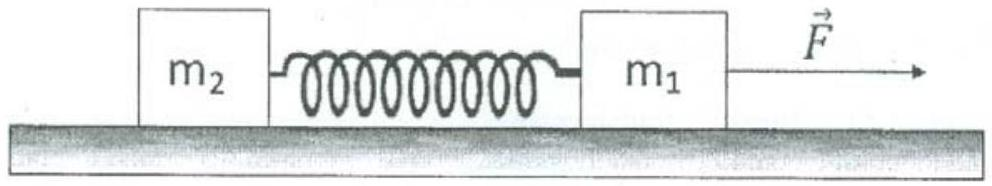
\includegraphics[width=0.4\linewidth]{images/2025_08_19_7d65f00c22d2f38e2422g-11}\\
a) $2,0 \mathrm{~N} ;$ b) $1,6 \mathrm{~N} ;$ c) $1,2 \mathrm{~N} ;$ d) $1,0 \mathrm{~N} ;$ e) $1,4 \mathrm{~N} ;$ f) $0,8 \mathrm{~N}$.

R15. Fie o forță constantă de valoare absolută $F$, care acționează asupra corpului 1 . Înainte de punerea în mişcare a corpului 2 , corpul 1 are o deplasare $d$, şi o viteză $v_{1}$. Folosind teorema variației energiei cinetice pentru corpul 1, folosind valorile lucrului mecanic efectuat de forța $F$, de forța elastică şi de forța de frecare, obținem:\\
$\frac{m_{1} v_{1}^{2}}{2}=F d-\frac{k d^{2}}{2}-\mu m_{1} g d$\\
Deplasarea $d$ a corpului 1 , aceeaşi cu alungirea resortului în momentul punerii în mişcare a corpului 2, corespunde egalizării forței de frecare $\mu m_{2} g$ de către forța de tracțiune forța elastică - $k d$, adică $\mu m_{2} g=k d$\\
Obținem: $\frac{m_{1} v_{1}^{2}}{2}=F d-\frac{\mu m_{2} g d}{2}-\mu m_{1} g d$, adică $F=\frac{m_{1} v_{1}^{2}}{2 d}+\frac{\mu m_{2} g}{2}+\mu m_{1} g$, aceasta fiind minimă atunci cînd corpul 1 are o viteză nulă: $F_{\min }=\mu\left(m_{1}+\frac{m_{2}}{2}\right) g=1,4 N$\\
Dacă forța $F$ nu este constantă, ea pune în mişcare lentă corpul 1 cînd are o valoare minimă egală cu $\mu m_{1} g$, şi creşte liniar cu deplasarea datorită creşterii liniare cu deplasarea - alungirea resortului - a forței elastice de reținere. În acest caz, forța medie este media aritmetică dintre forța minimă $\mu m_{1} g$ și forța maximă $F_{\max }$, iar lucrul mecanic al forței exterioare este $\frac{\mu m_{1} g+F_{\max }}{2} d$. Aplicînd teorema variației energiei cinetice pentru corpul 1, obținem: $\frac{m_{1} v_{1}^{2}}{2}=\frac{\mu m_{1} g+F_{\max }}{2} d-\frac{k d^{2}}{2}-\mu m_{1} g d$, cu condiția $\mu m_{2} g=k d$, şi cu precizarea că viteza finală $v_{1}$ a corpului 1 este nulă - mişcarea fiind lentă. $F_{\max }=\mu\left(m_{1}+m_{2}\right) g$. Acest rezultat se poate obține nu doar energetic, ci şi dinamic: după ce resortul capătă o alungire pentru care forța elastică corespunde forței de frecare a corpului 2 , resortul nu se mai deformează şi se comportă ca un fir inextensibil.\\
Comentariu: Forța medie în acest caz corespunde forței minime obținute anterior. În cazul forței constante, are loc mai întîi o accelerare a corpului 1, forța de tracțiune fiind inițial mai mare decît suma dintre forța de frecare și forța elastică, după care se produce încetinirea sa, suma dintre forța de frecare şi forța elastică devenind mai mare decît forța de tracțiune.\\
Comentariu 2. Care ar fi interesul practic al acestei probleme? Dacă forța $\vec{F}$ care acționează asupra corpului 1 este transmisă acestuia prin intermediul unui fir care nu ar suporta o tensiune egală cu $\mu\left(m_{1}+m_{2}\right) g=2 N$ (în sensul că s-ar rupe), nu ar putea fí mişcat din loc corpul 2 dacă s-ar acționa cu o forță variabilă, cum am văzut mai înainte. În\\
schimb, acționînd asupra corpului 1 cu o forță constantă cel puțin egală cu $\mu\left(m_{1}+\frac{m_{2}}{2}\right) g=1,4 N$, printr-un fir care suportă o tensiune de doar $1,4 N$, se reuşeşte punerea în mişcare a corpului 2 , dacă forța este constantă, aşa cum am văzut în primul caz studiat.

\section{Admitere F1 iulie 2016}

\begin{enumerate}
  \item O maşină termică funcționează după un ciclu Carnot între temperaturile $T_{1}=1200 \mathrm{~K}$ și $T_{2}=300 \mathrm{~K}$. Lucrul mecanic efectuat într-un ciclu este $L=3 \mathrm{~kJ}$. Căldura primită într-un ciclu este: ( 6 pet.)\\
a) 4 kJ ; b) $2,5 \mathrm{~kJ}$; c) 3 kJ ; d) 5 kJ ; e) 6 kJ ; f) $4,2 \mathrm{~kJ}$.
\end{enumerate}

R1. $\eta=1-\frac{T_{2}}{T_{1}}=\frac{T_{1}-T_{2}}{T_{1}}=\frac{L}{Q_{p}} \Rightarrow Q_{p}=L \frac{T_{1}}{T_{1}-T_{2}}=4 k J$\\
2. Un corp de masă $m=2 \mathrm{~kg}$ are impulsul $p=10 \mathrm{~kg} \cdot \mathrm{~m} / \mathrm{s}$. Energia cinetică a corpului este: ( 6 pct.)\\
a) 100 J ; b\\
b) 20 J ;\\
c) 15 J ;\\
d) 25 J ; e) 10 J ; f) 50 J .

R2. $E_{c}=\frac{p^{2}}{2 m}=25 J$\\
3. Randamentul unui circuit electric simplu este $60 \%$. Știind că intensitatea curentului de scurtcircuit al sursei are valoarea de 5A, intensitatea curentului electric prin circuit este: ( 6 pct.)\\
a) 6 A ; b) 1 A ; c) 3 A ; d) 5 A ; e) 4 A ; f) 2 A .

R3. $\eta=\frac{R}{R+r}=\frac{1}{1+\frac{r}{R}} \Rightarrow \frac{r}{R}=\frac{1-\eta}{\eta}$\\
$I_{S C}=\frac{E}{r}, I=\frac{E}{R+r}=\frac{E}{r} \cdot \frac{1}{1+\frac{R}{r}}=I_{S C} \cdot \frac{1}{1+\frac{R}{r}}=I_{S C} \cdot \frac{1}{1+\frac{\eta}{1-\eta}}=I_{S C} \cdot(1-\eta)=2 \mathrm{~A}$\\
4. Într-o transformare a unui gaz ideal temperatura creşte cu $20 \%$, iar volumul se reduce de 4 ori. Raportul dintre presiunea finală şi cea inițială este: ( 6 pct.)\\
a) 2,$5 ;$ b) $5 ;$ c) 3,$6 ;$ d) 1,$2 ;$ e) 4,$8 ;$ f) 8 .

R4. $\frac{p V}{T}=\frac{p_{0} V_{0}}{T_{0}} \Rightarrow \frac{p}{p_{0}}=\frac{V_{0}}{V} \cdot \frac{T}{T_{0}}=4,8$\\
5. Unitatea de măsură în SI pentru puterea mecanică este: ( 6 pct.)\\
a) $\frac{\mathrm{N}}{\mathrm{s}}$; b) J ; c) $\mathrm{J} \cdot \mathrm{s} ;$ d) $\mathrm{W} ;$ e) $\mathrm{N} ;$ f) $\mathrm{N} \cdot \mathrm{s}^{2}$.

R5. $[P]_{S I}=W$\\
6. Printr-un rezistor cu rezistența de $4 \Omega$ trece un curent electric cu intensitatea de 3 A . Tensiunea electrică la bornele rezistorului este: ( $\mathbf{6}$ pct.)\\
a) $\frac{3}{4} \mathrm{~V}$; b) 4 V ; c) 7 V ; d) $\frac{4}{3} \mathrm{~V}$; e) 1 V ; f) 12 V .

R6. $U=R I=12 \mathrm{~V}$\\
7. Utilizând notațiile din manualele de fizică, legea vitezei în mişcarea rẹctilinie uniform accelerată este: (6 pct.)\\
a) $a(t)=x \cdot t$; b) $a(t)=v_{0} \cdot t$; c) $v(t)=\frac{F}{m}$; d) $v(t)=m \cdot t^{2}$; e) $v(t)=v_{0}+a \cdot t$; f) $x(t)=x_{0}+a \cdot t$.

R7. $v(t)=v_{0}+a \cdot t$\\
8. Unitatea de măsură în SI pentru capacitatea calorică este: ( 6 pct.)\\
a) J; b) J/kg; c) J/mol; d) J/K; e) J.K; f) caloria.

R8. $[C]_{S I}=J / K$\\
9. O forţă de 2 N acționează asupra unui corp timp de 5 secunde. Variația impulsului corpului în acest interval de timp este: (6 pct.)\\
a) $40 \mathrm{~kg} \cdot \mathrm{~m} / \mathrm{s}$; b) $20 \mathrm{~kg} \cdot \mathrm{~m} / \mathrm{s}$; c)\\
$5 \mathrm{~kg} \cdot \mathrm{~m} / \mathrm{s}$; d\\
d) $25 \mathrm{~kg} \cdot \mathrm{~m} / \mathrm{s} ; \mathrm{e}$ )\\
$50 \mathrm{~kg} \cdot \mathrm{~m} / \mathrm{s} ; \mathrm{f})$\\
$10 \mathrm{~kg} \cdot \mathrm{~m} / \mathrm{s}$.

R9. $\Delta p=F \cdot \Delta t=10 \mathrm{~kg} \cdot \mathrm{~m} / \mathrm{s}$\\
10. Un număr de 10 cuburi identice fiecare cu latura de 20 cm și masa 2 kg se află unul lângă altul pe un plan orizontal. Pentru a aşeza cuburile unul peste altul astfel încât să formeze pe planul orizontal o coloană verticală, lucrul mecanic necesar este ( $g=10 \mathrm{~m} / \mathrm{s}^{2}$ ): ( 6 pct.)\\
a) 90 J ;\\
b) 180 J ; c) 40 J ;\\
d) 220 J ; e) 4 J ; f) 110 J .

R10. $L=\sum_{i=1}^{9} \mathrm{mg} \cdot \mathrm{il}=\mathrm{mgl} \cdot \sum_{i=1}^{9} i=45 \mathrm{mgl}=180 \mathrm{~J}$\\
11. Un corp cu masa de 20 kg este fabricat din fontă având căldura specifică $540 \mathrm{~J} /(\mathrm{kg} \cdot \mathrm{K})$. Cantitatea de căldură necesară încălzirii corpului cu $40^{\circ} \mathrm{C}$ este: ( 6 pct.)\\
a) 216 kJ ; b) 864 kJ ; c) 432 kJ ; d) 600 kJ ; e) 864 J ; f) 600 J .

R11. $Q=m c \Delta T=20 \mathrm{~kg} \cdot 540 \frac{\mathrm{~J}}{\mathrm{~kg} \cdot \mathrm{~K}} \cdot 40 \mathrm{~K}=432 \cdot 10^{3} \mathrm{~J}=432 \mathrm{~kJ}$\\
12. Un corp punctiform este aruncat de jos în sus în câmp gravitational ( $g=10 \mathrm{~m} / \mathrm{s}^{2}$ ) cu viteza $v_{0}=10 \mathrm{~m} / \mathrm{s}$. Inălțimea maximă la care ajunge corpul este: ( 6 pct.)\\
a) 4 m ; b)\\
b) 15 m ;\\
c) 1 m ;\\
d) 8 m ;\\
e) 5 m ; f\\
) 10 m .

R12. $h_{u}=\frac{v_{0}^{2}}{2 g}=5 \mathrm{~m}$\\
13. La bornele unui conductor cu rezistența electrică de $3 \Omega$ se aplică o tensiune electrică de 9 V . Sarcina electrică transportată printr-o secțiune transversală a conductorului în timp de 20 s este: ( 6 pct .)\\
a) 6 C ; b) 18 C ; c) 60 C ; d) 10 C ; e) 600 C ; f) 180 C .

R13. $q=I \cdot t=\frac{U}{R} \cdot t=60 \mathrm{C}$\\
14. Printr-un rezistor cu rezistenta de $15 \Omega$ trece un curent electric cu intensitatea de 2 A . Puterea disipată pe rezistor este: ( 6 pct.)\\
a) 15 W ; b)\\
b) 60 J ; c)\\
) 15 J ; d) $60 \mathrm{~W} ;$ e\\
e) 30 J ; f)\\
30 W .

R14. $P=R I^{2}=60 \mathrm{~W}$\\
15. Utilizând notaţiile din manualele de fizică legea lui Ohm pentru un circuit simplu este: (6 pct.)\\
a) $I=\frac{E}{R+r}$; b) $I=E \cdot r$; c) $I=E \cdot R$; d) $I=\frac{U^{2}}{R}$; e) $I=U \cdot R$; f) $I=E \cdot(R+r)$.

R15. $I=\frac{E}{R+r}$

\section{Admitere F iulie 2015}

\begin{enumerate}
  \item Un corp coboară fără frecare pe un plan înclinat de unghi $30^{\circ}$. Accelerația corpului este $\left(\mathrm{g}=10 \mathrm{~m} / \mathrm{s}^{2}\right)$ :
\end{enumerate}

\section*{Rezolvare}
Forța care acționează asupra corpului şi îi imprimă accelerația este componenta tangențială (paralelă cu planul înclinat) a greutății sale:\\
$G_{t}=m g \sin \alpha$\\
unde $\alpha$ este unghiul planului înclinat.\\
Aplicând expresia principiului al doilea al mecanicii, $\vec{F}=m \vec{a}$, rezultă $a=\frac{G_{t}}{m}=g \sin \alpha$, adică $a=10 \cdot \frac{1}{2}=5 \mathrm{~m} / \mathrm{s}^{2}$.\\
2. Puterea disipată pe un rezistor cu rezistența de $2 \Omega$ parcurs de un curent de 2 A este egală cu:

\section*{Rezolvare}
Conform definiției puterii electrice, $P=U I$ și legii lui Ohm pentru o porțiune de circuit, $U=R I$, rezultă $P=R I^{2}$, adică\\
$P=2 \cdot 4=8 \mathrm{~W}$.\\
3. Utilizând notațiile din manualele de fizică, ecuația termică de stare a gazului ideal este:

Rezolvare\\
$p V=\nu R T$\\
4. La legarea în serie sau în paralel a patru generatoare electrice identice, puterea disipată pe un rezistor este $P=160 \mathrm{~W}$. Puterea disipată de un singur generator pe acelaşi rezistor este:

\section*{Rezolvare}
La legarea în serie a celor patru generatoare identice, intensitatea curentului prin rezistorul de rezistență $R$, conectat la bornele acestei baterii de generatoare, este:\\
$I_{s}=\frac{4 E}{R+4 r}$, iar puterea disipată pe rezistor este $P=R I_{s}^{2}$.\\
La legarea generatoarelor în paralel, intensitatea curentului prin acelaşi rezistor de rezistență $R$, conectat la noua baterie de generatoare, este:\\
$I_{p}=\frac{E}{R+\frac{r}{4}}$, iar puterea disipată pe rezistor este $P=R I_{p}^{2}$.\\
Egalând puterile şi înlocuind expresiile $I_{s}$ şi $I_{p}$, rezultă $R=r$.\\
La conectarea rezistorului la un singur generator, intensitatea curentului prin circuit este $I=\frac{E}{R+r}$. Ținând cont că $R=r, I=\frac{E}{2 R}$, iar puterea disipată pe rezistor este $P^{\prime}=R I^{2}$, adică $P^{\prime}=\frac{E^{2}}{4 R}$.

Din $P=R I_{p}^{2}$ şi $R=r$ rezultă:\\
$P=R I_{p}^{2}=R\left(\frac{E}{R+\frac{r}{4}}\right)^{2}=R\left(\frac{E}{R+\frac{R}{4}}\right)^{2}=\frac{16}{25} \frac{E^{2}}{R}$,\\
adică $\frac{E^{2}}{R}=\frac{25}{16} P$. Ca urmare, $P^{\prime}=\frac{E^{2}}{4 R}=\frac{1}{4} \cdot \frac{25}{16} P=62,5 \mathrm{~W}$.\\
5. O masă de 150 g de gaz ideal ( $\mu=18 \mathrm{~g} / \mathrm{mol}$ ) suferă o transformare în care presiunea variază linear cu volumul. Gazul trece din starea $p_{1}=7 \cdot 10^{5} \mathrm{~Pa}, V_{1}=32$ litri în starea $p_{2}=10^{6} \mathrm{~Pa}, V_{2}=22$ litri. Temperatura maximă atinsă de gaz în această transformare este ( $R=8,3 \mathrm{~J} / \mathrm{mol} \cdot \mathrm{K}$ ):

\section*{Rezolvare}
Gazul suferă o transformare generală descrisă în coordonate ( $\mathrm{p}, \mathrm{V}$ ) prin legea $p(V)=a \cdot V+b$, în care $a=\frac{p_{2}-p_{1}}{V_{2}-V_{1}}$ şi $b=p_{1}-a \cdot V_{1}$, adică $a=-3 \cdot 10^{7} \mathrm{~Pa} / \mathrm{m}^{3}$ respectiv $b=16,6 \cdot 10^{5} \mathrm{~Pa}$. Înlocuind în această relație expresia presiunii $p=\frac{v R T}{V}$, așa cum rezultă din ecuația termică de stare a gazului ideal, se obține legea transformării generale a gazului în coordonate $(\mathrm{V}, \mathrm{T})$ : $T(V)=\frac{1}{v R}\left(a \cdot V^{2}+b \cdot V\right)$. Din condiția de extremum a acestei funcții, când volumul gazului este $V_{M}=-\frac{b}{2 a}$, el atinge temperatura maximă $T_{\text {max }}\left(V=V_{M}\right)=\frac{1}{v R}\left(\frac{-b^{2}}{4 a}\right)$ adică $T_{\text {max }}=332 \mathrm{~K}$.\\
6. O forță de 20 N acţionează asupra unui corp de masă $m=5 \mathrm{~kg}$ aflat în repaus pe o suprafață orizontală. Dacă se neglijează frecarea, spațiul parcurs de corp în primele 5 secunde de mişcare este:

\section*{Rezolvare}
Accelerația imprimată corpului rezultă din expresia principiului al doilea al mecanicii, $\vec{F}=m \vec{a}$, adică $a=\frac{F}{m}$.\\
Legea spațiului pentru corpul care pleacă din repaus este: $s=\frac{1}{2} a t^{2}$. Rezultă $s=\frac{1}{2} \frac{F}{m} t^{2}$, adică $s=\frac{1}{2} \frac{20}{5} \cdot 25=50 \mathrm{~m}$.\\
7. La capetele unui conductor de rezistență $2 \Omega$ se aplică o tensiune electrică de 4 V . Intensitatea curentului electric prin conductor este:

\section*{Rezolvare}
Aplicând legea lui Ohm pentru o porțiune de circuit, $I=\frac{U}{R}$, rezultă:\\
$I=\frac{4}{2}=2 \mathrm{~A}$.\\
8. Căldura disipată de un consumator cu rezistența de $20 \Omega$ străbătut de un curent de intensitate 2 A timp de 5 minute este:

\section*{Rezolvare}
Conform definiției $Q=W=U I t=R I^{2} t$, adică $Q=20 \cdot 4 \cdot(5 \cdot 60)=24000 \mathrm{~J}$, adică $Q=24 \mathrm{~kJ}$.\\
9. Volumul unui mol de gaz ideal la temperatura de 300 K şi presiunea de $10^{5} \mathbf{~ P a}$ ( $\mathbf{R} \boldsymbol{=} \mathbf{8 , 3} \mathbf{~ J} / \mathbf{m o l} \cdot \mathbf{K}$ ) este egal cu:

\section*{Rezolvare}
Din ecuația termică de stare a gazului ideal, $p V=v R T$, se obține $V=\frac{v R T}{p}$, adică $V=\frac{1 \cdot 8,3 \cdot 300}{10^{5}}=0,0249 \mathrm{~m}^{3}$.\\
10. Energia cinetică a unui corp de masă $m=2 \mathrm{~kg}$, care se mişcă cu viteza de $5 \mathrm{~m} / \mathrm{s}$, este:

\section*{Rezolvare}
Conform definiției energiei cinetice, $E_{c}=\frac{1}{2} m v^{2}$, rezultă $E_{c}=\frac{1}{2} 2 \cdot 25=25 \mathrm{~J}$.

\section*{11. Randamentul unui ciclu Carnot având temperaturile $T_{1}=500 \mathrm{~K}$ şi $T_{2}=300 \mathrm{~K}$ este:}
\section*{Rezolvare}
Randamentul ciclului Carnot, exprimat în funcție de temperaturile surselor caldă ( $T_{1}$ ) şi respectiv rece $\left(T_{2}\right)$, este $\eta=1-\frac{T_{2}}{T_{1}}$, adică : $\eta=1-\frac{300}{500}=0,4$.\\
12. Un gaz ideal aflat la presiunea de $10^{5} \mathrm{~Pa}$ suferă o transformare izocoră în urma căreia temperatura gazului se dublează. Presiunea gazului creşte cu:

\section*{Rezolvare}
Aplicând legea transformării izocore, $\frac{p}{T}=$ const., se obține $\frac{p_{1}}{T_{1}}=\frac{p_{2}}{2 T_{1}}$ şi $p_{2}=2 p_{1}$. Presiunea gazului creşte cu $\Delta p=p_{2}-p_{1}=p_{1}$, adică $\Delta p=10^{5} \mathrm{~Pa}$.\\
13. Temperatura unui kilogram de apă (cu căldura specifică $c=4185 \mathrm{~J} / \mathrm{kgK}$ ), care primeşte 0 cantitate de căldură de 83700 J , variază cu:

\section*{Rezolvare}
Din definiția căldurii specifice a unei substanțe, $c=\frac{Q}{m \Delta T}$, rezultă $\Delta T=\frac{Q}{m c}$, adică $\Delta T=\frac{83700}{1 \cdot 4185}=20 \mathrm{~K}$ sau $\Delta t=20^{\circ} \mathrm{C}$.\\
14. Utilizând notațiile din manualele de fizică, legea lui Ohm pentru circuitul simplu este:

Rezolvare\\
$I=\frac{E}{R+r}$\\
15. Unitatea de măsură în SI pentru impuls este:

Rezolvare\\
$[p]_{\mathrm{SI}}=\mathrm{kg} \cdot \mathrm{m} / \mathrm{s}$\\
16. Sub acțiunea unei forțe deformatoare $F$, alungirea absolută a unui resort cu constanta de elasticitate $\boldsymbol{k}$ este:

Rezolvare\\
Conform definiției, $F=k \cdot \Delta l$, adică\\
$\Delta l=\frac{F}{k}$.\\
17. Legea de mişcare a unui mobil este $x(t)=2 t^{2}-8 t+21$ (m). Coordonata $\boldsymbol{x}$ a mobilului la momentul de timp $t=2$ s este:

Rezolvare\\
Întroducând valoarea $t=2 \mathrm{~s}$ în legea de mişcare se obține:\\
$x(2)=2 \cdot 4-8 \cdot 2+21=13 \mathrm{~m}$.\\
18. Două rezistoare cu rezistențele de $2 \Omega$ şi respectiv $8 \Omega$ sunt legate în paralel. Rezistența echivalentă a grupării este:

Rezolvare\\
Din $\frac{1}{R_{p}}=\frac{1}{R_{1}}+\frac{1}{R_{2}}$ rezultă $R_{p}=\frac{R_{1} R_{2}}{R_{1}+R_{2}}$, adică $R_{p}=1,6 \Omega$.


\end{document}